\documentclass[preview]{standalone}

\usepackage{amsmath}
\usepackage{amssymb}
\usepackage{stellar}
\usepackage{definitions}
\usepackage{bettelini}
\usepackage{tikz}

\begin{document}

\id{green-gauss-theorem}
\genpage

\section{Planar Flux}

\begin{snippetproposition}{planar-divergence-flux-proposition}{Planar divergence formula}
    Let \(\Omega\subseteq\realnumbers^2\) be an admissible bounded domain,
    and let \(F=(A,B)\) be of class \(\mathcal C^1\) on a neighborhood of
    \(\overline\Omega\). Then
    \[
        \iint_\Omega(A_x+B_y)\,dx\,dy
        =\int_{\partial\Omega}(A,B)\cdot\nu_e\,d\sigma.
    \]
\end{snippetproposition}

\begin{snippet}{planar-flux-as-line-integral}
    Suppose \(\partial\Omega\) is positively parametrized by
    \(\gamma(t)=(x(t),y(t))\), so that \(\Omega\) remains to the left. The
    tangent is \((x',y')\), while the outward normal multiplied by arc
    length is
    \[
        \begin{pmatrix}0&1\\-1&0\end{pmatrix}
        \begin{pmatrix}x'\\y'\end{pmatrix}
        =\begin{pmatrix}y'\\-x'\end{pmatrix}.
    \]
    Therefore
    \begin{align*}
        \int_{\partial\Omega}(A,B)\cdot\nu_e\,d\sigma
        &=\integral[a][b]
        [A(x(t),y(t))y'(t)-B(x(t),y(t))x'(t)][t]\\
        &=\int_{\partial\Omega}-B\,dx+A\,dy.
    \end{align*}
\end{snippet}

\section{Green--Gauss Theorem}

\begin{snippettheorem}{classical-green-gauss-theorem}{Green--Gauss theorem}
    Let \(\Omega\subseteq\realnumbers^2\) be a bounded admissible domain
    with piecewise regular boundary, and let
    \(P,Q\in\mathcal C^1(U)\) on a neighborhood of
    \(\overline\Omega\). If \(\partial^+\Omega\) has positive orientation,
    then
    \[
        \int_{\partial^+\Omega}P\,dx+Q\,dy
        =\iint_\Omega(Q_x-P_y)\,dx\,dy.
    \]
\end{snippettheorem}

\begin{snippetproof}{classical-green-gauss-theorem-proof}{classical-green-gauss-theorem}{Green--Gauss theorem}
    Apply the planar divergence formula to the field \((A,B)=(Q,-P)\).
    Then
    \[
        A_x+B_y=Q_x-P_y,
    \]
    while the flux-to-line-integral identity gives
    \[
        \int_{\partial\Omega}(A,B)\cdot\nu_e\,d\sigma
        =\int_{\partial^+\Omega}P\,dx+Q\,dy.
    \]
    Combining the two identities proves the formula.
\end{snippetproof}

\begin{snippet}{green-gauss-multiply-connected-orientation}
    If \(\Omega\) has holes, positive orientation is understood component by
    component: the outer boundary is traversed counterclockwise and every
    inner boundary clockwise. In this way the domain always remains on the
    left of the moving boundary point.
\end{snippet}

\begin{snippetexample}{green-gauss-composite-boundary-example}{Line integral on a composite boundary}
    Let
    \[
        \Omega=\{(x,y):x\geq0,\ y\geq0,\ x+y\leq3,\ x^2+y^2\geq1\}.
    \]
    Compute
    \[
        \int_{\partial^+\Omega}y^2\,dx+x^2\,dy.
    \]

    \begin{center}
        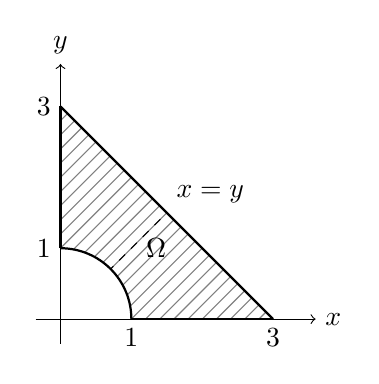
\begin{tikzpicture}[scale=0.9]
            \draw[->] (-0.35,0) -- (3.6,0) node[right] {\(x\)};
            \draw[->] (0,-0.35) -- (0,3.6) node[above] {\(y\)};

            \begin{scope}
                \clip
                    (0,1) --
                    (0,3) --
                    (3,0) --
                    (1,0)
                    arc[start angle=0,end angle=90,radius=1]
                    -- cycle;

                \foreach \t in {-3,-2.8,...,3}{
                    \draw[gray] (\t,0) -- ++(3,3);
                }

                \draw[dashed] (0,0) -- (3,3);
            \end{scope}

            \draw[thick] (0,3) -- (3,0);
            \draw[thick] (0,1) -- (0,3);
            \draw[thick] (1,0) -- (3,0);
            \draw[thick] (1,0)
                arc[start angle=0,end angle=90,radius=1];

            \node[left] at (0,1) {\(1\)};
            \node[left] at (0,3) {\(3\)};
            \node[below] at (1,0) {\(1\)};
            \node[below] at (3,0) {\(3\)};

            \node at (1.35,1.0) {\(\Omega\)};
            \node[above right] at (1.5,1.5) {\(x=y\)};
        \end{tikzpicture}
    \end{center}
\end{snippetexample}

\begin{snippetsolution}{green-gauss-composite-boundary-solution}{Line integral on a composite boundary}
    Take \(P=y^2\) and \(Q=x^2\). Green--Gauss gives
    \[
        \int_{\partial^+\Omega}y^2\,dx+x^2\,dy
        =\iint_\Omega2(x-y)\,dx\,dy.
    \]
    The domain is symmetric under interchange of \(x\) and \(y\), whereas
    the integrand changes sign. The two halves cancel, so the integral is
    zero.
\end{snippetsolution}

\end{document}
